\documentclass[1p]{elsarticle_modified}
%\bibliographystyle{elsarticle-num}

%\usepackage[colorlinks]{hyperref}
%\usepackage{abbrmath_seonhwa} %\Abb, \Ascr, \Acal ,\Abf, \Afrak
\usepackage{amsfonts}
\usepackage{amssymb}
\usepackage{amsmath}
\usepackage{amsthm}
\usepackage{scalefnt}
\usepackage{amsbsy}
\usepackage{kotex}
\usepackage{caption}
\usepackage{subfig}
\usepackage{color}
\usepackage{graphicx}
\usepackage{xcolor} %% white, black, red, green, blue, cyan, magenta, yellow
\usepackage{float}
\usepackage{setspace}
\usepackage{hyperref}

\usepackage{tikz}
\usetikzlibrary{arrows}

\usepackage{multirow}
\usepackage{array} % fixed length table
\usepackage{hhline}

%%%%%%%%%%%%%%%%%%%%%
\makeatletter
\renewcommand*\env@matrix[1][\arraystretch]{%
	\edef\arraystretch{#1}%
	\hskip -\arraycolsep
	\let\@ifnextchar\new@ifnextchar
	\array{*\c@MaxMatrixCols c}}
\makeatother %https://tex.stackexchange.com/questions/14071/how-can-i-increase-the-line-spacing-in-a-matrix
%%%%%%%%%%%%%%%

\usepackage[normalem]{ulem}

\newcommand{\msout}[1]{\ifmmode\text{\sout{\ensuremath{#1}}}\else\sout{#1}\fi}
%SOURCE: \msout is \stkout macro in https://tex.stackexchange.com/questions/20609/strikeout-in-math-mode

\newcommand{\cancel}[1]{
	\ifmmode
	{\color{red}\msout{#1}}
	\else
	{\color{red}\sout{#1}}
	\fi
}

\newcommand{\add}[1]{
	{\color{blue}\uwave{#1}}
}

\newcommand{\replace}[2]{
	\ifmmode
	{\color{red}\msout{#1}}{\color{blue}\uwave{#2}}
	\else
	{\color{red}\sout{#1}}{\color{blue}\uwave{#2}}
	\fi
}

\newcommand{\Sol}{\mathcal{S}} %segment
\newcommand{\D}{D} %diagram
\newcommand{\A}{\mathcal{A}} %arc


%%%%%%%%%%%%%%%%%%%%%%%%%%%%%5 test

\def\sl{\operatorname{\textup{SL}}(2,\Cbb)}
\def\psl{\operatorname{\textup{PSL}}(2,\Cbb)}
\def\quan{\mkern 1mu \triangleright \mkern 1mu}

\theoremstyle{definition}
\newtheorem{thm}{Theorem}[section]
\newtheorem{prop}[thm]{Proposition}
\newtheorem{lem}[thm]{Lemma}
\newtheorem{ques}[thm]{Question}
\newtheorem{cor}[thm]{Corollary}
\newtheorem{defn}[thm]{Definition}
\newtheorem{exam}[thm]{Example}
\newtheorem{rmk}[thm]{Remark}
\newtheorem{alg}[thm]{Algorithm}

\newcommand{\I}{\sqrt{-1}}
\begin{document}

%\begin{frontmatter}
%
%\title{Boundary parabolic representations of knots up to 8 crossings}
%
%%% Group authors per affiliation:
%\author{Yunhi Cho} 
%\address{Department of Mathematics, University of Seoul, Seoul, Korea}
%\ead{yhcho@uos.ac.kr}
%
%
%\author{Seonhwa Kim} %\fnref{s_kim}}
%\address{Center for Geometry and Physics, Institute for Basic Science, Pohang, 37673, Korea}
%\ead{ryeona17@ibs.re.kr}
%
%\author{Hyuk Kim}
%\address{Department of Mathematical Sciences, Seoul National University, Seoul 08826, Korea}
%\ead{hyukkim@snu.ac.kr}
%
%\author{Seokbeom Yoon}
%\address{Department of Mathematical Sciences, Seoul National University, Seoul, 08826,  Korea}
%\ead{sbyoon15@snu.ac.kr}
%
%\begin{abstract}
%We find all boundary parabolic representation of knots up to 8 crossings.
%
%\end{abstract}
%\begin{keyword}
%    \MSC[2010] 57M25 
%\end{keyword}
%
%\end{frontmatter}

%\linenumbers
%\tableofcontents
%
\newcommand\colored[1]{\textcolor{white}{\rule[-0.35ex]{0.8em}{1.4ex}}\kern-0.8em\color{red} #1}%
%\newcommand\colored[1]{\textcolor{white}{ #1}\kern-2.17ex	\textcolor{white}{ #1}\kern-1.81ex	\textcolor{white}{ #1}\kern-2.15ex\color{red}#1	}

{\Large $\underline{12a_{0556}~(K12a_{0556})}$}

\setlength{\tabcolsep}{10pt}
\renewcommand{\arraystretch}{1.6}
\vspace{1cm}\begin{tabular}{m{100pt}>{\centering\arraybackslash}m{274pt}}
\multirow{5}{120pt}{
	\centering
	\includegraphics[width=112pt]{../../../GIT/diagram.site/Diagrams/png/1357_12a_0556.png}\\
\ \ \ A knot diagram\footnotemark}&
\allowdisplaybreaks
\textbf{Linearized knot diagam} \\
\cline{2-2}
 &
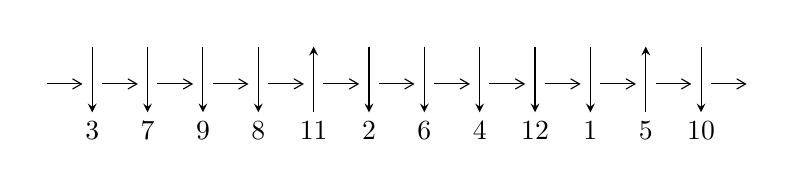
\begin{tikzpicture}[x=20pt, y=17pt]
	% nodes
	\node (C0) at (0, 0) {};
	\node (C1) at (1, 0) {};
	\node (C1U) at (1, +1) {};
	\node (C1D) at (1, -1) {3};

	\node (C2) at (2, 0) {};
	\node (C2U) at (2, +1) {};
	\node (C2D) at (2, -1) {7};

	\node (C3) at (3, 0) {};
	\node (C3U) at (3, +1) {};
	\node (C3D) at (3, -1) {9};

	\node (C4) at (4, 0) {};
	\node (C4U) at (4, +1) {};
	\node (C4D) at (4, -1) {8};

	\node (C5) at (5, 0) {};
	\node (C5U) at (5, +1) {};
	\node (C5D) at (5, -1) {11};

	\node (C6) at (6, 0) {};
	\node (C6U) at (6, +1) {};
	\node (C6D) at (6, -1) {2};

	\node (C7) at (7, 0) {};
	\node (C7U) at (7, +1) {};
	\node (C7D) at (7, -1) {6};

	\node (C8) at (8, 0) {};
	\node (C8U) at (8, +1) {};
	\node (C8D) at (8, -1) {4};

	\node (C9) at (9, 0) {};
	\node (C9U) at (9, +1) {};
	\node (C9D) at (9, -1) {12};

	\node (C10) at (10, 0) {};
	\node (C10U) at (10, +1) {};
	\node (C10D) at (10, -1) {1};

	\node (C11) at (11, 0) {};
	\node (C11U) at (11, +1) {};
	\node (C11D) at (11, -1) {5};

	\node (C12) at (12, 0) {};
	\node (C12U) at (12, +1) {};
	\node (C12D) at (12, -1) {10};
	\node (C13) at (13, 0) {};

	% arrows
	\draw[->,>={angle 60}]
	(C0) edge (C1) (C1) edge (C2) (C2) edge (C3) (C3) edge (C4) (C4) edge (C5) (C5) edge (C6) (C6) edge (C7) (C7) edge (C8) (C8) edge (C9) (C9) edge (C10) (C10) edge (C11) (C11) edge (C12) (C12) edge (C13) ;	\draw[->,>=stealth]
	(C1U) edge (C1D) (C2U) edge (C2D) (C3U) edge (C3D) (C4U) edge (C4D) (C5D) edge (C5U) (C6U) edge (C6D) (C7U) edge (C7D) (C8U) edge (C8D) (C9U) edge (C9D) (C10U) edge (C10D) (C11D) edge (C11U) (C12U) edge (C12D) ;
	\end{tikzpicture} \\
\hhline{~~} \\& 
\textbf{Solving Sequence} \\ \cline{2-2} 
 &
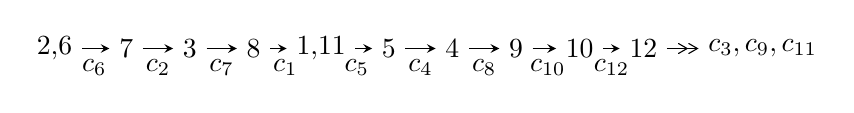
\begin{tikzpicture}[x=23pt, y=7pt]
	% node
	\node (A0) at (-1/8, 0) {2,6};
	\node (A1) at (1, 0) {7};
	\node (A2) at (2, 0) {3};
	\node (A3) at (3, 0) {8};
	\node (A4) at (65/16, 0) {1,11};
	\node (A5) at (41/8, 0) {5};
	\node (A6) at (49/8, 0) {4};
	\node (A7) at (57/8, 0) {9};
	\node (A8) at (65/8, 0) {10};
	\node (A9) at (73/8, 0) {12};
	\node (C1) at (1/2, -1) {$c_{6}$};
	\node (C2) at (3/2, -1) {$c_{2}$};
	\node (C3) at (5/2, -1) {$c_{7}$};
	\node (C4) at (7/2, -1) {$c_{1}$};
	\node (C5) at (37/8, -1) {$c_{5}$};
	\node (C6) at (45/8, -1) {$c_{4}$};
	\node (C7) at (53/8, -1) {$c_{8}$};
	\node (C8) at (61/8, -1) {$c_{10}$};
	\node (C9) at (69/8, -1) {$c_{12}$};
	\node (A10) at (11, 0) {$c_{3},c_{9},c_{11}$};

	% edge
	\draw[->,>=stealth]	
	(A0) edge (A1) (A1) edge (A2) (A2) edge (A3) (A3) edge (A4) (A4) edge (A5) (A5) edge (A6) (A6) edge (A7) (A7) edge (A8) (A8) edge (A9) ;
	\draw[->>,>={angle 60}]	
	(A9) edge (A10);
\end{tikzpicture} \\ 

\end{tabular} \\

\footnotetext{
The image of knot diagram is generated by the software ``\textbf{Draw programme}" developed by Andrew Bartholomew(\url{http://www.layer8.co.uk/maths/draw/index.htm\#Running-draw}), where we modified some parts for our purpose(\url{https://github.com/CATsTAILs/LinksPainter}).
}\phantom \\ \newline 
\centering \textbf{Ideals for irreducible components\footnotemark of $X_{\text{par}}$} 
 
\begin{align*}
I^u_{1}&=\langle 
1.07057\times10^{77} u^{84}-1.50389\times10^{77} u^{83}+\cdots+2.53839\times10^{77} b+9.88146\times10^{77},\\
\phantom{I^u_{1}}&\phantom{= \langle  }4.68186\times10^{77} u^{84}-4.98399\times10^{77} u^{83}+\cdots+7.61518\times10^{77} a+1.56488\times10^{78},\;u^{85}-2 u^{84}+\cdots+3 u-9\rangle \\
I^u_{2}&=\langle 
b,\;u^4- u^2+a-2 u+1,\;u^5+u^4- u^2+u+1\rangle \\
I^u_{3}&=\langle 
- u^3 a- u^2 a+2 u^3+a u- u^2+2 b- u+1,\;-2 u^3 a+u^2 a+3 u^3+a^2+a u- u^2- a-2 u,\;u^4- u^2+1\rangle \\
\\
\end{align*}
\raggedright * 3 irreducible components of $\dim_{\mathbb{C}}=0$, with total 98 representations.\\
\footnotetext{All coefficients of polynomials are rational numbers. But the coefficients are sometimes approximated in decimal forms when there is not enough margin.}
\newpage
\renewcommand{\arraystretch}{1}
\centering \section*{I. $I^u_{1}= \langle 1.07\times10^{77} u^{84}-1.50\times10^{77} u^{83}+\cdots+2.54\times10^{77} b+9.88\times10^{77},\;4.68\times10^{77} u^{84}-4.98\times10^{77} u^{83}+\cdots+7.62\times10^{77} a+1.56\times10^{78},\;u^{85}-2 u^{84}+\cdots+3 u-9 \rangle$}
\flushleft \textbf{(i) Arc colorings}\\
\begin{tabular}{m{7pt} m{180pt} m{7pt} m{180pt} }
\flushright $a_{2}=$&$\begin{pmatrix}0\\u\end{pmatrix}$ \\
\flushright $a_{6}=$&$\begin{pmatrix}1\\0\end{pmatrix}$ \\
\flushright $a_{7}=$&$\begin{pmatrix}1\\u^2\end{pmatrix}$ \\
\flushright $a_{3}=$&$\begin{pmatrix}- u\\- u^3+u\end{pmatrix}$ \\
\flushright $a_{8}=$&$\begin{pmatrix}- u^2+1\\u^2\end{pmatrix}$ \\
\flushright $a_{1}=$&$\begin{pmatrix}u^3\\u^5- u^3+u\end{pmatrix}$ \\
\flushright $a_{11}=$&$\begin{pmatrix}-0.614806 u^{84}+0.654481 u^{83}+\cdots+9.36540 u-2.05495\\-0.421753 u^{84}+0.592456 u^{83}+\cdots-1.27756 u-3.89280\end{pmatrix}$ \\
\flushright $a_{5}=$&$\begin{pmatrix}0.681235 u^{84}-0.376546 u^{83}+\cdots-7.23243 u+7.03410\\-0.191650 u^{84}-0.675652 u^{83}+\cdots+8.48193 u+7.43904\end{pmatrix}$ \\
\flushright $a_{4}=$&$\begin{pmatrix}1.86822 u^{84}-0.943208 u^{83}+\cdots-12.5547 u+7.89357\\-0.0907235 u^{84}-1.88072 u^{83}+\cdots+17.6608 u+14.6758\end{pmatrix}$ \\
\flushright $a_{9}=$&$\begin{pmatrix}1.63065 u^{84}-3.35202 u^{83}+\cdots+13.0436 u+22.5528\\-2.79323 u^{84}+3.46800 u^{83}+\cdots-2.28892 u-16.8140\end{pmatrix}$ \\
\flushright $a_{10}=$&$\begin{pmatrix}0.699998 u^{84}-1.53125 u^{83}+\cdots+14.4778 u+10.2525\\-1.30758 u^{84}+1.53849 u^{83}+\cdots-1.30083 u-10.6368\end{pmatrix}$ \\
\flushright $a_{12}=$&$\begin{pmatrix}-1.80393 u^{84}+3.41357 u^{83}+\cdots-3.48625 u-22.2978\\3.09725 u^{84}-3.65415 u^{83}+\cdots+0.275477 u+18.2000\end{pmatrix}$\\&\end{tabular}
\flushleft \textbf{(ii) Obstruction class $= -1$}\\~\\
\flushleft \textbf{(iii) Cusp Shapes $= 0.269673 u^{84}-0.693788 u^{83}+\cdots+4.57663 u-2.13190$}\\~\\
\newpage\renewcommand{\arraystretch}{1}
\flushleft \textbf{(iv) u-Polynomials at the component}\newline \\
\begin{tabular}{m{50pt}|m{274pt}}
Crossings & \hspace{64pt}u-Polynomials at each crossing \\
\hline $$\begin{aligned}c_{1},c_{7}\end{aligned}$$&$\begin{aligned}
&u^{85}+28 u^{84}+\cdots+1107 u+81
\end{aligned}$\\
\hline $$\begin{aligned}c_{2},c_{6}\end{aligned}$$&$\begin{aligned}
&u^{85}-2 u^{84}+\cdots+3 u-9
\end{aligned}$\\
\hline $$\begin{aligned}c_{3},c_{4},c_{8}\end{aligned}$$&$\begin{aligned}
&u^{85}-2 u^{84}+\cdots+144 u-36
\end{aligned}$\\
\hline $$\begin{aligned}c_{5},c_{11}\end{aligned}$$&$\begin{aligned}
&u^{85}+u^{84}+\cdots-96 u-32
\end{aligned}$\\
\hline $$\begin{aligned}c_{9},c_{10},c_{12}\end{aligned}$$&$\begin{aligned}
&u^{85}-10 u^{84}+\cdots+17 u-1
\end{aligned}$\\
\hline
\end{tabular}\\~\\
\newpage\renewcommand{\arraystretch}{1}
\flushleft \textbf{(v) Riley Polynomials at the component}\newline \\
\begin{tabular}{m{50pt}|m{274pt}}
Crossings & \hspace{64pt}Riley Polynomials at each crossing \\
\hline $$\begin{aligned}c_{1},c_{7}\end{aligned}$$&$\begin{aligned}
&y^{85}+64 y^{84}+\cdots+485595 y-6561
\end{aligned}$\\
\hline $$\begin{aligned}c_{2},c_{6}\end{aligned}$$&$\begin{aligned}
&y^{85}-28 y^{84}+\cdots+1107 y-81
\end{aligned}$\\
\hline $$\begin{aligned}c_{3},c_{4},c_{8}\end{aligned}$$&$\begin{aligned}
&y^{85}+80 y^{84}+\cdots+16776 y-1296
\end{aligned}$\\
\hline $$\begin{aligned}c_{5},c_{11}\end{aligned}$$&$\begin{aligned}
&y^{85}+45 y^{84}+\cdots+22016 y-1024
\end{aligned}$\\
\hline $$\begin{aligned}c_{9},c_{10},c_{12}\end{aligned}$$&$\begin{aligned}
&y^{85}-80 y^{84}+\cdots-91 y-1
\end{aligned}$\\
\hline
\end{tabular}\\~\\
\newpage\flushleft \textbf{(vi) Complex Volumes and Cusp Shapes}
$$\begin{array}{c|c|c}  
\text{Solutions to }I^u_{1}& \I (\text{vol} + \sqrt{-1}CS) & \text{Cusp shape}\\
 \hline 
\begin{aligned}
u &= -0.998621\phantom{ +0.000000I} \\
a &= -0.294335\phantom{ +0.000000I} \\
b &= \phantom{-}1.06804\phantom{ +0.000000I}\end{aligned}
 & -5.84228\phantom{ +0.000000I} & -16.3890\phantom{ +0.000000I} \\ \hline\begin{aligned}
u &= -0.806816 + 0.599615 I \\
a &= \phantom{-}0.703510 + 0.591628 I \\
b &= -0.319657 + 0.693146 I\end{aligned}
 & -0.43718 + 2.02855 I & \phantom{-0.000000 } 0 \\ \hline\begin{aligned}
u &= -0.806816 - 0.599615 I \\
a &= \phantom{-}0.703510 - 0.591628 I \\
b &= -0.319657 - 0.693146 I\end{aligned}
 & -0.43718 - 2.02855 I & \phantom{-0.000000 } 0 \\ \hline\begin{aligned}
u &= \phantom{-}0.984839 + 0.081448 I \\
a &= \phantom{-}0.48248 + 1.60444 I \\
b &= -0.198977 + 1.034500 I\end{aligned}
 & -3.82226 - 2.23236 I & -15.8479 + 4.6950 I \\ \hline\begin{aligned}
u &= \phantom{-}0.984839 - 0.081448 I \\
a &= \phantom{-}0.48248 - 1.60444 I \\
b &= -0.198977 - 1.034500 I\end{aligned}
 & -3.82226 + 2.23236 I & -15.8479 - 4.6950 I \\ \hline\begin{aligned}
u &= \phantom{-}1.016480 + 0.146739 I \\
a &= \phantom{-}0.131558 - 0.758826 I \\
b &= -1.033670 - 0.298635 I\end{aligned}
 & -2.02964 - 3.37819 I & \phantom{-0.000000 } 0 \\ \hline\begin{aligned}
u &= \phantom{-}1.016480 - 0.146739 I \\
a &= \phantom{-}0.131558 + 0.758826 I \\
b &= -1.033670 + 0.298635 I\end{aligned}
 & -2.02964 + 3.37819 I & \phantom{-0.000000 } 0 \\ \hline\begin{aligned}
u &= \phantom{-}0.709986 + 0.663321 I \\
a &= \phantom{-}2.20996 + 0.27167 I \\
b &= -0.850401 + 0.427141 I\end{aligned}
 & -1.108310 + 0.109986 I & -8.00000 + 0. I\phantom{ +0.000000I} \\ \hline\begin{aligned}
u &= \phantom{-}0.709986 - 0.663321 I \\
a &= \phantom{-}2.20996 - 0.27167 I \\
b &= -0.850401 - 0.427141 I\end{aligned}
 & -1.108310 - 0.109986 I & -8.00000 + 0. I\phantom{ +0.000000I} \\ \hline\begin{aligned}
u &= -0.900145 + 0.529083 I \\
a &= \phantom{-}5.92919 - 1.06315 I \\
b &= -0.309938 + 0.046527 I\end{aligned}
 & -0.08293 + 2.04372 I & \phantom{-0.000000 } 0\\
 \hline 
 \end{array}$$\newpage$$\begin{array}{c|c|c}  
\text{Solutions to }I^u_{1}& \I (\text{vol} + \sqrt{-1}CS) & \text{Cusp shape}\\
 \hline 
\begin{aligned}
u &= -0.900145 - 0.529083 I \\
a &= \phantom{-}5.92919 + 1.06315 I \\
b &= -0.309938 - 0.046527 I\end{aligned}
 & -0.08293 - 2.04372 I & \phantom{-0.000000 } 0 \\ \hline\begin{aligned}
u &= -0.724002 + 0.754097 I \\
a &= -0.922405 + 0.673843 I \\
b &= \phantom{-}0.555009 - 0.921380 I\end{aligned}
 & \phantom{-}1.77796 - 1.79805 I & \phantom{-0.000000 } 0 \\ \hline\begin{aligned}
u &= -0.724002 - 0.754097 I \\
a &= -0.922405 - 0.673843 I \\
b &= \phantom{-}0.555009 + 0.921380 I\end{aligned}
 & \phantom{-}1.77796 + 1.79805 I & \phantom{-0.000000 } 0 \\ \hline\begin{aligned}
u &= \phantom{-}0.775319 + 0.522980 I \\
a &= -0.458774 + 0.800072 I \\
b &= \phantom{-}0.235131 - 0.116553 I\end{aligned}
 & \phantom{-}1.78078 - 2.10361 I & \phantom{-0.000000 -}0. + 4.46892 I \\ \hline\begin{aligned}
u &= \phantom{-}0.775319 - 0.522980 I \\
a &= -0.458774 - 0.800072 I \\
b &= \phantom{-}0.235131 + 0.116553 I\end{aligned}
 & \phantom{-}1.78078 + 2.10361 I & \phantom{-0.000000 } 0. - 4.46892 I \\ \hline\begin{aligned}
u &= \phantom{-}0.268293 + 0.888731 I \\
a &= -0.732829 + 0.719131 I \\
b &= \phantom{-}0.581673 - 1.021050 I\end{aligned}
 & \phantom{-}0.28979 - 6.12813 I & -7.02703 + 5.51860 I \\ \hline\begin{aligned}
u &= \phantom{-}0.268293 - 0.888731 I \\
a &= -0.732829 - 0.719131 I \\
b &= \phantom{-}0.581673 + 1.021050 I\end{aligned}
 & \phantom{-}0.28979 + 6.12813 I & -7.02703 - 5.51860 I \\ \hline\begin{aligned}
u &= -0.711753 + 0.806285 I \\
a &= -1.84218 + 0.24993 I \\
b &= \phantom{-}1.26596 + 0.66556 I\end{aligned}
 & \phantom{-}4.32861 - 2.99556 I & \phantom{-0.000000 } 0 \\ \hline\begin{aligned}
u &= -0.711753 - 0.806285 I \\
a &= -1.84218 - 0.24993 I \\
b &= \phantom{-}1.26596 - 0.66556 I\end{aligned}
 & \phantom{-}4.32861 + 2.99556 I & \phantom{-0.000000 } 0 \\ \hline\begin{aligned}
u &= \phantom{-}0.867038 + 0.661822 I \\
a &= -1.308520 + 0.434436 I \\
b &= -0.06260 - 1.87617 I\end{aligned}
 & -5.78886 - 2.56710 I & \phantom{-0.000000 } 0\\
 \hline 
 \end{array}$$\newpage$$\begin{array}{c|c|c}  
\text{Solutions to }I^u_{1}& \I (\text{vol} + \sqrt{-1}CS) & \text{Cusp shape}\\
 \hline 
\begin{aligned}
u &= \phantom{-}0.867038 - 0.661822 I \\
a &= -1.308520 - 0.434436 I \\
b &= -0.06260 + 1.87617 I\end{aligned}
 & -5.78886 + 2.56710 I & \phantom{-0.000000 } 0 \\ \hline\begin{aligned}
u &= \phantom{-}0.759915 + 0.787119 I \\
a &= -0.139375 - 0.369733 I \\
b &= \phantom{-}0.543133 + 1.290540 I\end{aligned}
 & \phantom{-}5.21127 - 0.29207 I & \phantom{-0.000000 } 0 \\ \hline\begin{aligned}
u &= \phantom{-}0.759915 - 0.787119 I \\
a &= -0.139375 + 0.369733 I \\
b &= \phantom{-}0.543133 - 1.290540 I\end{aligned}
 & \phantom{-}5.21127 + 0.29207 I & \phantom{-0.000000 } 0 \\ \hline\begin{aligned}
u &= -0.674977 + 0.862853 I \\
a &= \phantom{-}0.848112 - 1.114180 I \\
b &= -0.606952 + 1.131660 I\end{aligned}
 & -3.29308 - 5.51174 I & \phantom{-0.000000 } 0 \\ \hline\begin{aligned}
u &= -0.674977 - 0.862853 I \\
a &= \phantom{-}0.848112 + 1.114180 I \\
b &= -0.606952 - 1.131660 I\end{aligned}
 & -3.29308 + 5.51174 I & \phantom{-0.000000 } 0 \\ \hline\begin{aligned}
u &= -0.996557 + 0.465595 I \\
a &= \phantom{-}1.127330 + 0.051322 I \\
b &= \phantom{-}0.09960 - 1.43805 I\end{aligned}
 & -8.63067 + 1.50287 I & \phantom{-0.000000 } 0 \\ \hline\begin{aligned}
u &= -0.996557 - 0.465595 I \\
a &= \phantom{-}1.127330 - 0.051322 I \\
b &= \phantom{-}0.09960 + 1.43805 I\end{aligned}
 & -8.63067 - 1.50287 I & \phantom{-0.000000 } 0 \\ \hline\begin{aligned}
u &= \phantom{-}0.693699 + 0.854594 I \\
a &= \phantom{-}0.694895 + 0.626975 I \\
b &= -0.729780 - 1.197990 I\end{aligned}
 & \phantom{-}7.72360 + 5.45340 I & \phantom{-0.000000 } 0 \\ \hline\begin{aligned}
u &= \phantom{-}0.693699 - 0.854594 I \\
a &= \phantom{-}0.694895 - 0.626975 I \\
b &= -0.729780 + 1.197990 I\end{aligned}
 & \phantom{-}7.72360 - 5.45340 I & \phantom{-0.000000 } 0 \\ \hline\begin{aligned}
u &= -0.873454 + 0.207048 I \\
a &= \phantom{-}1.70854 - 0.67125 I \\
b &= -0.20097 - 1.51805 I\end{aligned}
 & -8.29116 + 1.11793 I & -14.9646 + 1.4167 I\\
 \hline 
 \end{array}$$\newpage$$\begin{array}{c|c|c}  
\text{Solutions to }I^u_{1}& \I (\text{vol} + \sqrt{-1}CS) & \text{Cusp shape}\\
 \hline 
\begin{aligned}
u &= -0.873454 - 0.207048 I \\
a &= \phantom{-}1.70854 + 0.67125 I \\
b &= -0.20097 + 1.51805 I\end{aligned}
 & -8.29116 - 1.11793 I & -14.9646 - 1.4167 I \\ \hline\begin{aligned}
u &= \phantom{-}0.631492 + 0.905031 I \\
a &= -0.944080 - 0.902830 I \\
b &= \phantom{-}0.83894 + 1.21192 I\end{aligned}
 & \phantom{-}2.45406 + 10.41200 I & \phantom{-0.000000 } 0 \\ \hline\begin{aligned}
u &= \phantom{-}0.631492 - 0.905031 I \\
a &= -0.944080 + 0.902830 I \\
b &= \phantom{-}0.83894 - 1.21192 I\end{aligned}
 & \phantom{-}2.45406 - 10.41200 I & \phantom{-0.000000 } 0 \\ \hline\begin{aligned}
u &= -0.886138 + 0.123069 I \\
a &= -0.92190 - 1.99206 I \\
b &= -0.053379 - 0.976140 I\end{aligned}
 & -0.667588 + 1.025160 I & -12.54308 - 0.08033 I \\ \hline\begin{aligned}
u &= -0.886138 - 0.123069 I \\
a &= -0.92190 + 1.99206 I \\
b &= -0.053379 + 0.976140 I\end{aligned}
 & -0.667588 - 1.025160 I & -12.54308 + 0.08033 I \\ \hline\begin{aligned}
u &= \phantom{-}0.850775 + 0.712293 I \\
a &= \phantom{-}0.798573 + 0.967990 I \\
b &= -0.612070 - 0.514601 I\end{aligned}
 & \phantom{-}2.60791 - 2.73509 I & \phantom{-0.000000 } 0 \\ \hline\begin{aligned}
u &= \phantom{-}0.850775 - 0.712293 I \\
a &= \phantom{-}0.798573 - 0.967990 I \\
b &= -0.612070 + 0.514601 I\end{aligned}
 & \phantom{-}2.60791 + 2.73509 I & \phantom{-0.000000 } 0 \\ \hline\begin{aligned}
u &= -1.093410 + 0.191489 I \\
a &= -0.21969 + 1.48130 I \\
b &= \phantom{-}0.482351 + 1.025410 I\end{aligned}
 & \phantom{-}0.65643 + 5.42394 I & \phantom{-0.000000 } 0 \\ \hline\begin{aligned}
u &= -1.093410 - 0.191489 I \\
a &= -0.21969 - 1.48130 I \\
b &= \phantom{-}0.482351 - 1.025410 I\end{aligned}
 & \phantom{-}0.65643 - 5.42394 I & \phantom{-0.000000 } 0 \\ \hline\begin{aligned}
u &= -0.922652 + 0.626826 I \\
a &= -1.48767 + 0.81968 I \\
b &= \phantom{-}0.235613 + 0.929059 I\end{aligned}
 & -0.82236 + 2.80542 I & \phantom{-0.000000 } 0\\
 \hline 
 \end{array}$$\newpage$$\begin{array}{c|c|c}  
\text{Solutions to }I^u_{1}& \I (\text{vol} + \sqrt{-1}CS) & \text{Cusp shape}\\
 \hline 
\begin{aligned}
u &= -0.922652 - 0.626826 I \\
a &= -1.48767 - 0.81968 I \\
b &= \phantom{-}0.235613 - 0.929059 I\end{aligned}
 & -0.82236 - 2.80542 I & \phantom{-0.000000 } 0 \\ \hline\begin{aligned}
u &= \phantom{-}1.105020 + 0.170837 I \\
a &= -0.762252 - 0.928102 I \\
b &= \phantom{-}0.412640 - 1.334080 I\end{aligned}
 & -10.32480 - 5.23736 I & \phantom{-0.000000 } 0 \\ \hline\begin{aligned}
u &= \phantom{-}1.105020 - 0.170837 I \\
a &= -0.762252 + 0.928102 I \\
b &= \phantom{-}0.412640 + 1.334080 I\end{aligned}
 & -10.32480 + 5.23736 I & \phantom{-0.000000 } 0 \\ \hline\begin{aligned}
u &= \phantom{-}1.034710 + 0.424655 I \\
a &= \phantom{-}0.678821 + 0.419020 I \\
b &= \phantom{-}0.453832 + 0.596946 I\end{aligned}
 & \phantom{-}2.03787 - 1.45102 I & \phantom{-0.000000 } 0 \\ \hline\begin{aligned}
u &= \phantom{-}1.034710 - 0.424655 I \\
a &= \phantom{-}0.678821 - 0.419020 I \\
b &= \phantom{-}0.453832 - 0.596946 I\end{aligned}
 & \phantom{-}2.03787 + 1.45102 I & \phantom{-0.000000 } 0 \\ \hline\begin{aligned}
u &= \phantom{-}0.887489 + 0.698307 I \\
a &= -1.81058 + 0.09319 I \\
b &= \phantom{-}0.549211 - 0.690031 I\end{aligned}
 & \phantom{-}2.49176 - 2.67187 I & \phantom{-0.000000 } 0 \\ \hline\begin{aligned}
u &= \phantom{-}0.887489 - 0.698307 I \\
a &= -1.81058 - 0.09319 I \\
b &= \phantom{-}0.549211 + 0.690031 I\end{aligned}
 & \phantom{-}2.49176 + 2.67187 I & \phantom{-0.000000 } 0 \\ \hline\begin{aligned}
u &= \phantom{-}0.759240 + 0.855036 I \\
a &= -0.365619 - 1.259310 I \\
b &= \phantom{-}0.353657 + 0.964749 I\end{aligned}
 & -1.327970 - 0.401840 I & \phantom{-0.000000 } 0 \\ \hline\begin{aligned}
u &= \phantom{-}0.759240 - 0.855036 I \\
a &= -0.365619 + 1.259310 I \\
b &= \phantom{-}0.353657 - 0.964749 I\end{aligned}
 & -1.327970 + 0.401840 I & \phantom{-0.000000 } 0 \\ \hline\begin{aligned}
u &= \phantom{-}0.967500 + 0.663999 I \\
a &= -1.16043 - 1.12609 I \\
b &= \phantom{-}1.042120 + 0.405267 I\end{aligned}
 & -1.88422 - 5.29403 I & \phantom{-0.000000 } 0\\
 \hline 
 \end{array}$$\newpage$$\begin{array}{c|c|c}  
\text{Solutions to }I^u_{1}& \I (\text{vol} + \sqrt{-1}CS) & \text{Cusp shape}\\
 \hline 
\begin{aligned}
u &= \phantom{-}0.967500 - 0.663999 I \\
a &= -1.16043 + 1.12609 I \\
b &= \phantom{-}1.042120 - 0.405267 I\end{aligned}
 & -1.88422 + 5.29403 I & \phantom{-0.000000 } 0 \\ \hline\begin{aligned}
u &= -0.826690 + 0.842297 I \\
a &= \phantom{-}1.264590 - 0.276686 I \\
b &= -1.032940 - 0.397310 I\end{aligned}
 & \phantom{-}10.14220 + 0.91099 I & \phantom{-0.000000 } 0 \\ \hline\begin{aligned}
u &= -0.826690 - 0.842297 I \\
a &= \phantom{-}1.264590 + 0.276686 I \\
b &= -1.032940 + 0.397310 I\end{aligned}
 & \phantom{-}10.14220 - 0.91099 I & \phantom{-0.000000 } 0 \\ \hline\begin{aligned}
u &= -0.979456 + 0.706863 I \\
a &= \phantom{-}1.99453 - 0.39746 I \\
b &= -0.548510 - 1.048100 I\end{aligned}
 & \phantom{-}1.00480 + 7.36064 I & \phantom{-0.000000 } 0 \\ \hline\begin{aligned}
u &= -0.979456 - 0.706863 I \\
a &= \phantom{-}1.99453 + 0.39746 I \\
b &= -0.548510 + 1.048100 I\end{aligned}
 & \phantom{-}1.00480 - 7.36064 I & \phantom{-0.000000 } 0 \\ \hline\begin{aligned}
u &= -1.200290 + 0.153170 I \\
a &= \phantom{-}0.338551 - 0.939110 I \\
b &= -0.631973 - 1.218280 I\end{aligned}
 & -4.88195 + 9.31216 I & \phantom{-0.000000 } 0 \\ \hline\begin{aligned}
u &= -1.200290 - 0.153170 I \\
a &= \phantom{-}0.338551 + 0.939110 I \\
b &= -0.631973 + 1.218280 I\end{aligned}
 & -4.88195 - 9.31216 I & \phantom{-0.000000 } 0 \\ \hline\begin{aligned}
u &= \phantom{-}0.967716 + 0.732266 I \\
a &= \phantom{-}1.56362 + 0.49238 I \\
b &= -0.42587 + 1.36774 I\end{aligned}
 & \phantom{-}4.57399 - 5.44218 I & \phantom{-0.000000 } 0 \\ \hline\begin{aligned}
u &= \phantom{-}0.967716 - 0.732266 I \\
a &= \phantom{-}1.56362 - 0.49238 I \\
b &= -0.42587 - 1.36774 I\end{aligned}
 & \phantom{-}4.57399 + 5.44218 I & \phantom{-0.000000 } 0 \\ \hline\begin{aligned}
u &= -1.000590 + 0.727268 I \\
a &= \phantom{-}0.73771 - 1.21462 I \\
b &= -1.35820 + 0.57857 I\end{aligned}
 & \phantom{-}3.44867 + 8.76620 I & \phantom{-0.000000 } 0\\
 \hline 
 \end{array}$$\newpage$$\begin{array}{c|c|c}  
\text{Solutions to }I^u_{1}& \I (\text{vol} + \sqrt{-1}CS) & \text{Cusp shape}\\
 \hline 
\begin{aligned}
u &= -1.000590 - 0.727268 I \\
a &= \phantom{-}0.73771 + 1.21462 I \\
b &= -1.35820 - 0.57857 I\end{aligned}
 & \phantom{-}3.44867 - 8.76620 I & \phantom{-0.000000 } 0 \\ \hline\begin{aligned}
u &= -0.946573 + 0.803204 I \\
a &= -0.739615 + 0.818673 I \\
b &= \phantom{-}1.022410 - 0.261567 I\end{aligned}
 & \phantom{-}9.77457 + 5.21014 I & \phantom{-0.000000 } 0 \\ \hline\begin{aligned}
u &= -0.946573 - 0.803204 I \\
a &= -0.739615 - 0.818673 I \\
b &= \phantom{-}1.022410 + 0.261567 I\end{aligned}
 & \phantom{-}9.77457 - 5.21014 I & \phantom{-0.000000 } 0 \\ \hline\begin{aligned}
u &= \phantom{-}0.995841 + 0.763155 I \\
a &= \phantom{-}1.69209 - 0.43161 I \\
b &= -0.479759 + 1.044820 I\end{aligned}
 & -2.07273 - 5.62883 I & \phantom{-0.000000 } 0 \\ \hline\begin{aligned}
u &= \phantom{-}0.995841 - 0.763155 I \\
a &= \phantom{-}1.69209 + 0.43161 I \\
b &= -0.479759 - 1.044820 I\end{aligned}
 & -2.07273 + 5.62883 I & \phantom{-0.000000 } 0 \\ \hline\begin{aligned}
u &= \phantom{-}0.147072 + 0.728915 I \\
a &= \phantom{-}0.683793 - 0.110743 I \\
b &= -0.656032 + 0.815272 I\end{aligned}
 & \phantom{-}4.76220 - 2.53471 I & -1.46695 + 3.47281 I \\ \hline\begin{aligned}
u &= \phantom{-}0.147072 - 0.728915 I \\
a &= \phantom{-}0.683793 + 0.110743 I \\
b &= -0.656032 - 0.815272 I\end{aligned}
 & \phantom{-}4.76220 + 2.53471 I & -1.46695 - 3.47281 I \\ \hline\begin{aligned}
u &= -0.150086 + 0.725683 I \\
a &= \phantom{-}0.54471 + 1.31256 I \\
b &= -0.202918 - 1.187480 I\end{aligned}
 & -6.11100 + 2.42065 I & -11.51467 - 3.42821 I \\ \hline\begin{aligned}
u &= -0.150086 - 0.725683 I \\
a &= \phantom{-}0.54471 - 1.31256 I \\
b &= -0.202918 + 1.187480 I\end{aligned}
 & -6.11100 - 2.42065 I & -11.51467 + 3.42821 I \\ \hline\begin{aligned}
u &= \phantom{-}1.027010 + 0.742791 I \\
a &= -1.86187 - 0.57547 I \\
b &= \phantom{-}0.67693 - 1.27703 I\end{aligned}
 & \phantom{-}6.70036 - 11.40770 I & \phantom{-0.000000 } 0\\
 \hline 
 \end{array}$$\newpage$$\begin{array}{c|c|c}  
\text{Solutions to }I^u_{1}& \I (\text{vol} + \sqrt{-1}CS) & \text{Cusp shape}\\
 \hline 
\begin{aligned}
u &= \phantom{-}1.027010 - 0.742791 I \\
a &= -1.86187 + 0.57547 I \\
b &= \phantom{-}0.67693 + 1.27703 I\end{aligned}
 & \phantom{-}6.70036 + 11.40770 I & \phantom{-0.000000 } 0 \\ \hline\begin{aligned}
u &= -0.730565\phantom{ +0.000000I} \\
a &= \phantom{-}0.0171409\phantom{ +0.000000I} \\
b &= -0.401918\phantom{ +0.000000I}\end{aligned}
 & -1.07739\phantom{ +0.000000I} & -9.03050\phantom{ +0.000000I} \\ \hline\begin{aligned}
u &= -1.038750 + 0.736760 I \\
a &= -2.04598 + 0.10778 I \\
b &= \phantom{-}0.672589 + 1.206980 I\end{aligned}
 & -4.41235 + 11.46610 I & \phantom{-0.000000 } 0 \\ \hline\begin{aligned}
u &= -1.038750 - 0.736760 I \\
a &= -2.04598 - 0.10778 I \\
b &= \phantom{-}0.672589 - 1.206980 I\end{aligned}
 & -4.41235 - 11.46610 I & \phantom{-0.000000 } 0 \\ \hline\begin{aligned}
u &= \phantom{-}1.166100 + 0.516708 I \\
a &= -0.690535 + 0.225074 I \\
b &= -0.402473 - 1.048200 I\end{aligned}
 & -2.57120 + 1.00877 I & \phantom{-0.000000 } 0 \\ \hline\begin{aligned}
u &= \phantom{-}1.166100 - 0.516708 I \\
a &= -0.690535 - 0.225074 I \\
b &= -0.402473 + 1.048200 I\end{aligned}
 & -2.57120 - 1.00877 I & \phantom{-0.000000 } 0 \\ \hline\begin{aligned}
u &= \phantom{-}1.073740 + 0.736661 I \\
a &= \phantom{-}2.00421 + 0.50463 I \\
b &= -0.84789 + 1.28835 I\end{aligned}
 & \phantom{-}1.0897 - 16.4761 I & \phantom{-0.000000 } 0 \\ \hline\begin{aligned}
u &= \phantom{-}1.073740 - 0.736661 I \\
a &= \phantom{-}2.00421 - 0.50463 I \\
b &= -0.84789 - 1.28835 I\end{aligned}
 & \phantom{-}1.0897 + 16.4761 I & \phantom{-0.000000 } 0 \\ \hline\begin{aligned}
u &= -0.942740 + 0.934437 I \\
a &= -0.350351 - 0.512078 I \\
b &= \phantom{-}0.061691 + 0.565881 I\end{aligned}
 & \phantom{-}8.96196 + 3.42091 I & \phantom{-0.000000 } 0 \\ \hline\begin{aligned}
u &= -0.942740 - 0.934437 I \\
a &= -0.350351 + 0.512078 I \\
b &= \phantom{-}0.061691 - 0.565881 I\end{aligned}
 & \phantom{-}8.96196 - 3.42091 I & \phantom{-0.000000 } 0\\
 \hline 
 \end{array}$$\newpage$$\begin{array}{c|c|c}  
\text{Solutions to }I^u_{1}& \I (\text{vol} + \sqrt{-1}CS) & \text{Cusp shape}\\
 \hline 
\begin{aligned}
u &= -0.111200 + 0.545459 I \\
a &= -1.08297 - 1.20293 I \\
b &= \phantom{-}0.699790 - 0.645759 I\end{aligned}
 & \phantom{-}1.50806 + 1.20124 I & -5.48394 - 0.07233 I \\ \hline\begin{aligned}
u &= -0.111200 - 0.545459 I \\
a &= -1.08297 + 1.20293 I \\
b &= \phantom{-}0.699790 + 0.645759 I\end{aligned}
 & \phantom{-}1.50806 - 1.20124 I & -5.48394 + 0.07233 I \\ \hline\begin{aligned}
u &= -0.193935 + 0.335714 I \\
a &= -1.051420 - 0.253121 I \\
b &= \phantom{-}0.180316 + 0.662567 I\end{aligned}
 & -0.404941 + 0.957173 I & -6.94345 - 7.00511 I \\ \hline\begin{aligned}
u &= -0.193935 - 0.335714 I \\
a &= -1.051420 + 0.253121 I \\
b &= \phantom{-}0.180316 - 0.662567 I\end{aligned}
 & -0.404941 - 0.957173 I & -6.94345 + 7.00511 I \\ \hline\begin{aligned}
u &= \phantom{-}0.311045\phantom{ +0.000000I} \\
a &= \phantom{-}3.80168\phantom{ +0.000000I} \\
b &= -0.461365\phantom{ +0.000000I}\end{aligned}
 & -2.06404\phantom{ +0.000000I} & -1.31720\phantom{ +0.000000I}\\
 \hline 
 \end{array}$$\newpage\newpage\renewcommand{\arraystretch}{1}
\centering \section*{II. $I^u_{2}= \langle b,\;u^4- u^2+a-2 u+1,\;u^5+u^4- u^2+u+1 \rangle$}
\flushleft \textbf{(i) Arc colorings}\\
\begin{tabular}{m{7pt} m{180pt} m{7pt} m{180pt} }
\flushright $a_{2}=$&$\begin{pmatrix}0\\u\end{pmatrix}$ \\
\flushright $a_{6}=$&$\begin{pmatrix}1\\0\end{pmatrix}$ \\
\flushright $a_{7}=$&$\begin{pmatrix}1\\u^2\end{pmatrix}$ \\
\flushright $a_{3}=$&$\begin{pmatrix}- u\\- u^3+u\end{pmatrix}$ \\
\flushright $a_{8}=$&$\begin{pmatrix}- u^2+1\\u^2\end{pmatrix}$ \\
\flushright $a_{1}=$&$\begin{pmatrix}u^3\\- u^4- u^3+u^2-1\end{pmatrix}$ \\
\flushright $a_{11}=$&$\begin{pmatrix}- u^4+u^2+2 u-1\\0\end{pmatrix}$ \\
\flushright $a_{5}=$&$\begin{pmatrix}1\\0\end{pmatrix}$ \\
\flushright $a_{4}=$&$\begin{pmatrix}u^4- u^2+1\\- u^4\end{pmatrix}$ \\
\flushright $a_{9}=$&$\begin{pmatrix}- u^3\\u^4+u^3- u^2+1\end{pmatrix}$ \\
\flushright $a_{10}=$&$\begin{pmatrix}- u^4- u^3+u^2+2 u-1\\u^4+u^3- u^2+1\end{pmatrix}$ \\
\flushright $a_{12}=$&$\begin{pmatrix}- u^4+u^2+2 u-1\\0\end{pmatrix}$\\&\end{tabular}
\flushleft \textbf{(ii) Obstruction class $= 1$}\\~\\
\flushleft \textbf{(iii) Cusp Shapes $= -9 u^4- u^3+2 u^2+4 u-17$}\\~\\
\newpage\renewcommand{\arraystretch}{1}
\flushleft \textbf{(iv) u-Polynomials at the component}\newline \\
\begin{tabular}{m{50pt}|m{274pt}}
Crossings & \hspace{64pt}u-Polynomials at each crossing \\
\hline $$\begin{aligned}c_{1},c_{3},c_{4}\end{aligned}$$&$\begin{aligned}
&u^5- u^4+4 u^3-3 u^2+3 u-1
\end{aligned}$\\
\hline $$\begin{aligned}c_{2}\end{aligned}$$&$\begin{aligned}
&u^5- u^4+u^2+u-1
\end{aligned}$\\
\hline $$\begin{aligned}c_{5},c_{11}\end{aligned}$$&$\begin{aligned}
&u^5
\end{aligned}$\\
\hline $$\begin{aligned}c_{6}\end{aligned}$$&$\begin{aligned}
&u^5+u^4- u^2+u+1
\end{aligned}$\\
\hline $$\begin{aligned}c_{7},c_{8}\end{aligned}$$&$\begin{aligned}
&u^5+u^4+4 u^3+3 u^2+3 u+1
\end{aligned}$\\
\hline $$\begin{aligned}c_{9},c_{10}\end{aligned}$$&$\begin{aligned}
&(u-1)^5
\end{aligned}$\\
\hline $$\begin{aligned}c_{12}\end{aligned}$$&$\begin{aligned}
&(u+1)^5
\end{aligned}$\\
\hline
\end{tabular}\\~\\
\newpage\renewcommand{\arraystretch}{1}
\flushleft \textbf{(v) Riley Polynomials at the component}\newline \\
\begin{tabular}{m{50pt}|m{274pt}}
Crossings & \hspace{64pt}Riley Polynomials at each crossing \\
\hline $$\begin{aligned}c_{1},c_{3},c_{4}\\c_{7},c_{8}\end{aligned}$$&$\begin{aligned}
&y^5+7 y^4+16 y^3+13 y^2+3 y-1
\end{aligned}$\\
\hline $$\begin{aligned}c_{2},c_{6}\end{aligned}$$&$\begin{aligned}
&y^5- y^4+4 y^3-3 y^2+3 y-1
\end{aligned}$\\
\hline $$\begin{aligned}c_{5},c_{11}\end{aligned}$$&$\begin{aligned}
&y^5
\end{aligned}$\\
\hline $$\begin{aligned}c_{9},c_{10},c_{12}\end{aligned}$$&$\begin{aligned}
&(y-1)^5
\end{aligned}$\\
\hline
\end{tabular}\\~\\
\newpage\flushleft \textbf{(vi) Complex Volumes and Cusp Shapes}
$$\begin{array}{c|c|c}  
\text{Solutions to }I^u_{2}& \I (\text{vol} + \sqrt{-1}CS) & \text{Cusp shape}\\
 \hline 
\begin{aligned}
u &= \phantom{-}0.758138 + 0.584034 I \\
a &= \phantom{-}1.47956 + 1.63976 I \\
b &= \phantom{-0.000000 } 0\end{aligned}
 & \phantom{-}0.17487 - 2.21397 I & -6.59361 - 0.42541 I \\ \hline\begin{aligned}
u &= \phantom{-}0.758138 - 0.584034 I \\
a &= \phantom{-}1.47956 - 1.63976 I \\
b &= \phantom{-0.000000 } 0\end{aligned}
 & \phantom{-}0.17487 + 2.21397 I & -6.59361 + 0.42541 I \\ \hline\begin{aligned}
u &= -0.935538 + 0.903908 I \\
a &= \phantom{-}0.044146 + 0.313338 I \\
b &= \phantom{-0.000000 } 0\end{aligned}
 & \phantom{-}9.31336 + 3.33174 I & \phantom{-}3.61324 + 0.36944 I \\ \hline\begin{aligned}
u &= -0.935538 - 0.903908 I \\
a &= \phantom{-}0.044146 - 0.313338 I \\
b &= \phantom{-0.000000 } 0\end{aligned}
 & \phantom{-}9.31336 - 3.33174 I & \phantom{-}3.61324 - 0.36944 I \\ \hline\begin{aligned}
u &= -0.645200\phantom{ +0.000000I} \\
a &= -2.04741\phantom{ +0.000000I} \\
b &= \phantom{-0.000000 } 0\end{aligned}
 & -2.52712\phantom{ +0.000000I} & -20.0390\phantom{ +0.000000I}\\
 \hline 
 \end{array}$$\newpage\newpage\renewcommand{\arraystretch}{1}
\centering \section*{III. $I^u_{3}= \langle - u^3 a- u^2 a+2 u^3+a u- u^2+2 b- u+1,\;-2 u^3 a+u^2 a+3 u^3+a^2+a u- u^2- a-2 u,\;u^4- u^2+1 \rangle$}
\flushleft \textbf{(i) Arc colorings}\\
\begin{tabular}{m{7pt} m{180pt} m{7pt} m{180pt} }
\flushright $a_{2}=$&$\begin{pmatrix}0\\u\end{pmatrix}$ \\
\flushright $a_{6}=$&$\begin{pmatrix}1\\0\end{pmatrix}$ \\
\flushright $a_{7}=$&$\begin{pmatrix}1\\u^2\end{pmatrix}$ \\
\flushright $a_{3}=$&$\begin{pmatrix}- u\\- u^3+u\end{pmatrix}$ \\
\flushright $a_{8}=$&$\begin{pmatrix}- u^2+1\\u^2\end{pmatrix}$ \\
\flushright $a_{1}=$&$\begin{pmatrix}u^3\\0\end{pmatrix}$ \\
\flushright $a_{11}=$&$\begin{pmatrix}a\\\frac{1}{2} u^3 a- u^3+\cdots+\frac{1}{2} u-\frac{1}{2}\end{pmatrix}$ \\
\flushright $a_{5}=$&$\begin{pmatrix}-\frac{1}{2} u^2 a-\frac{1}{2} u^3+\cdots+\frac{1}{2} a-\frac{1}{2}\\-\frac{1}{2} u^3 a+\frac{1}{2} u^2 a+\cdots+\frac{1}{2} u-\frac{3}{2}\end{pmatrix}$ \\
\flushright $a_{4}=$&$\begin{pmatrix}-\frac{1}{2} u^2 a-\frac{1}{2} u^3+\cdots+\frac{1}{2} a-\frac{1}{2}\\-\frac{1}{2} u^3 a- u^3+\cdots+\frac{3}{2} u-\frac{3}{2}\end{pmatrix}$ \\
\flushright $a_{9}=$&$\begin{pmatrix}\frac{1}{2} u^2 a-\frac{3}{2} u^3+\cdots-\frac{1}{2} a+\frac{1}{2}\\-\frac{1}{2} u^3 a+2 u^3+\cdots-\frac{1}{2} u+\frac{1}{2}\end{pmatrix}$ \\
\flushright $a_{10}=$&$\begin{pmatrix}-\frac{1}{2} u^3 a+u^3+\cdots+a+\frac{1}{2}\\\frac{1}{2} u^3 a- u^3+\cdots+\frac{1}{2} u-\frac{1}{2}\end{pmatrix}$ \\
\flushright $a_{12}=$&$\begin{pmatrix}\frac{1}{2} u^3 a-\frac{3}{2} u^3+\cdots-\frac{1}{2} a+\frac{5}{2} u\\-\frac{1}{2} u^3 a+2 u^3+\cdots-\frac{1}{2} u+\frac{1}{2}\end{pmatrix}$\\&\end{tabular}
\flushleft \textbf{(ii) Obstruction class $= 1$}\\~\\
\flushleft \textbf{(iii) Cusp Shapes $= 4 u^2-12$}\\~\\
\newpage\renewcommand{\arraystretch}{1}
\flushleft \textbf{(iv) u-Polynomials at the component}\newline \\
\begin{tabular}{m{50pt}|m{274pt}}
Crossings & \hspace{64pt}u-Polynomials at each crossing \\
\hline $$\begin{aligned}c_{1}\end{aligned}$$&$\begin{aligned}
&(u^2- u+1)^4
\end{aligned}$\\
\hline $$\begin{aligned}c_{2},c_{6}\end{aligned}$$&$\begin{aligned}
&(u^4- u^2+1)^2
\end{aligned}$\\
\hline $$\begin{aligned}c_{3},c_{4},c_{8}\end{aligned}$$&$\begin{aligned}
&(u^2+1)^4
\end{aligned}$\\
\hline $$\begin{aligned}c_{5},c_{11}\end{aligned}$$&$\begin{aligned}
&(u^4+3 u^2+1)^2
\end{aligned}$\\
\hline $$\begin{aligned}c_{7}\end{aligned}$$&$\begin{aligned}
&(u^2+u+1)^4
\end{aligned}$\\
\hline $$\begin{aligned}c_{9},c_{10}\end{aligned}$$&$\begin{aligned}
&(u^2+u-1)^4
\end{aligned}$\\
\hline $$\begin{aligned}c_{12}\end{aligned}$$&$\begin{aligned}
&(u^2- u-1)^4
\end{aligned}$\\
\hline
\end{tabular}\\~\\
\newpage\renewcommand{\arraystretch}{1}
\flushleft \textbf{(v) Riley Polynomials at the component}\newline \\
\begin{tabular}{m{50pt}|m{274pt}}
Crossings & \hspace{64pt}Riley Polynomials at each crossing \\
\hline $$\begin{aligned}c_{1},c_{7}\end{aligned}$$&$\begin{aligned}
&(y^2+y+1)^4
\end{aligned}$\\
\hline $$\begin{aligned}c_{2},c_{6}\end{aligned}$$&$\begin{aligned}
&(y^2- y+1)^4
\end{aligned}$\\
\hline $$\begin{aligned}c_{3},c_{4},c_{8}\end{aligned}$$&$\begin{aligned}
&(y+1)^8
\end{aligned}$\\
\hline $$\begin{aligned}c_{5},c_{11}\end{aligned}$$&$\begin{aligned}
&(y^2+3 y+1)^4
\end{aligned}$\\
\hline $$\begin{aligned}c_{9},c_{10},c_{12}\end{aligned}$$&$\begin{aligned}
&(y^2-3 y+1)^4
\end{aligned}$\\
\hline
\end{tabular}\\~\\
\newpage\flushleft \textbf{(vi) Complex Volumes and Cusp Shapes}
$$\begin{array}{c|c|c}  
\text{Solutions to }I^u_{3}& \I (\text{vol} + \sqrt{-1}CS) & \text{Cusp shape}\\
 \hline 
\begin{aligned}
u &= \phantom{-}0.866025 + 0.500000 I \\
a &= \phantom{-}1.344250 - 0.092242 I \\
b &= \phantom{-0.000000 -}0.618034 I\end{aligned}
 & \phantom{-}0.65797 - 2.02988 I & -10.00000 + 3.46410 I \\ \hline\begin{aligned}
u &= \phantom{-}0.866025 + 0.500000 I \\
a &= -1.71028 + 0.72622 I \\
b &= \phantom{-0.000000 } -1.61803 I\end{aligned}
 & -7.23771 - 2.02988 I & -10.00000 + 3.46410 I \\ \hline\begin{aligned}
u &= \phantom{-}0.866025 - 0.500000 I \\
a &= \phantom{-}1.344250 + 0.092242 I \\
b &= \phantom{-0.000000 } -0.618034 I\end{aligned}
 & \phantom{-}0.65797 + 2.02988 I & -10.00000 - 3.46410 I \\ \hline\begin{aligned}
u &= \phantom{-}0.866025 - 0.500000 I \\
a &= -1.71028 - 0.72622 I \\
b &= \phantom{-0.000000 -}1.61803 I\end{aligned}
 & -7.23771 + 2.02988 I & -10.00000 - 3.46410 I \\ \hline\begin{aligned}
u &= -0.866025 + 0.500000 I \\
a &= \phantom{-}1.092240 - 0.344250 I \\
b &= \phantom{-0.000000 } -1.61803 I\end{aligned}
 & -7.23771 + 2.02988 I & -10.00000 - 3.46410 I \\ \hline\begin{aligned}
u &= -0.866025 + 0.500000 I \\
a &= \phantom{-}0.27378 + 2.71028 I \\
b &= \phantom{-0.000000 -}0.618034 I\end{aligned}
 & \phantom{-}0.65797 + 2.02988 I & -10.00000 - 3.46410 I \\ \hline\begin{aligned}
u &= -0.866025 - 0.500000 I \\
a &= \phantom{-}1.092240 + 0.344250 I \\
b &= \phantom{-0.000000 -}1.61803 I\end{aligned}
 & -7.23771 - 2.02988 I & -10.00000 + 3.46410 I \\ \hline\begin{aligned}
u &= -0.866025 - 0.500000 I \\
a &= \phantom{-}0.27378 - 2.71028 I \\
b &= \phantom{-0.000000 } -0.618034 I\end{aligned}
 & \phantom{-}0.65797 - 2.02988 I & -10.00000 + 3.46410 I\\
 \hline 
 \end{array}$$\newpage
\newpage\renewcommand{\arraystretch}{1}
\centering \section*{ IV. u-Polynomials}
\begin{tabular}{m{50pt}|m{274pt}}
Crossings & \hspace{64pt}u-Polynomials at each crossing \\
\hline $$\begin{aligned}c_{1}\end{aligned}$$&$\begin{aligned}
&(u^2- u+1)^4(u^5- u^4+4 u^3-3 u^2+3 u-1)\\
&\cdot(u^{85}+28 u^{84}+\cdots+1107 u+81)
\end{aligned}$\\
\hline $$\begin{aligned}c_{2}\end{aligned}$$&$\begin{aligned}
&((u^4- u^2+1)^2)(u^5- u^4+u^2+u-1)(u^{85}-2 u^{84}+\cdots+3 u-9)
\end{aligned}$\\
\hline $$\begin{aligned}c_{3},c_{4}\end{aligned}$$&$\begin{aligned}
&((u^2+1)^4)(u^5- u^4+\cdots+3 u-1)(u^{85}-2 u^{84}+\cdots+144 u-36)
\end{aligned}$\\
\hline $$\begin{aligned}c_{5},c_{11}\end{aligned}$$&$\begin{aligned}
&u^5(u^4+3 u^2+1)^2(u^{85}+u^{84}+\cdots-96 u-32)
\end{aligned}$\\
\hline $$\begin{aligned}c_{6}\end{aligned}$$&$\begin{aligned}
&((u^4- u^2+1)^2)(u^5+u^4- u^2+u+1)(u^{85}-2 u^{84}+\cdots+3 u-9)
\end{aligned}$\\
\hline $$\begin{aligned}c_{7}\end{aligned}$$&$\begin{aligned}
&(u^2+u+1)^4(u^5+u^4+4 u^3+3 u^2+3 u+1)\\
&\cdot(u^{85}+28 u^{84}+\cdots+1107 u+81)
\end{aligned}$\\
\hline $$\begin{aligned}c_{8}\end{aligned}$$&$\begin{aligned}
&((u^2+1)^4)(u^5+u^4+\cdots+3 u+1)(u^{85}-2 u^{84}+\cdots+144 u-36)
\end{aligned}$\\
\hline $$\begin{aligned}c_{9},c_{10}\end{aligned}$$&$\begin{aligned}
&((u-1)^5)(u^2+u-1)^4(u^{85}-10 u^{84}+\cdots+17 u-1)
\end{aligned}$\\
\hline $$\begin{aligned}c_{12}\end{aligned}$$&$\begin{aligned}
&((u+1)^5)(u^2- u-1)^4(u^{85}-10 u^{84}+\cdots+17 u-1)
\end{aligned}$\\
\hline
\end{tabular}\newpage\renewcommand{\arraystretch}{1}
\centering \section*{ V. Riley Polynomials}
\begin{tabular}{m{50pt}|m{274pt}}
Crossings & \hspace{64pt}Riley Polynomials at each crossing \\
\hline $$\begin{aligned}c_{1},c_{7}\end{aligned}$$&$\begin{aligned}
&(y^2+y+1)^4(y^5+7 y^4+16 y^3+13 y^2+3 y-1)\\
&\cdot(y^{85}+64 y^{84}+\cdots+485595 y-6561)
\end{aligned}$\\
\hline $$\begin{aligned}c_{2},c_{6}\end{aligned}$$&$\begin{aligned}
&(y^2- y+1)^4(y^5- y^4+4 y^3-3 y^2+3 y-1)\\
&\cdot(y^{85}-28 y^{84}+\cdots+1107 y-81)
\end{aligned}$\\
\hline $$\begin{aligned}c_{3},c_{4},c_{8}\end{aligned}$$&$\begin{aligned}
&(y+1)^8(y^5+7 y^4+16 y^3+13 y^2+3 y-1)\\
&\cdot(y^{85}+80 y^{84}+\cdots+16776 y-1296)
\end{aligned}$\\
\hline $$\begin{aligned}c_{5},c_{11}\end{aligned}$$&$\begin{aligned}
&y^5(y^2+3 y+1)^4(y^{85}+45 y^{84}+\cdots+22016 y-1024)
\end{aligned}$\\
\hline $$\begin{aligned}c_{9},c_{10},c_{12}\end{aligned}$$&$\begin{aligned}
&((y-1)^5)(y^2-3 y+1)^4(y^{85}-80 y^{84}+\cdots-91 y-1)
\end{aligned}$\\
\hline
\end{tabular}
\vskip 2pc
\end{document}